%!TEX root = project.tex

\chapter{Technology Review}
About seven to ten pages.
\begin{itemize}
\item Describe each of the technologies you used at a conceptual level. Standards, Database Model (e.g. MongoDB, CouchDB), XMl, WSDL, JSON, JAXP.
\item Use references (IEEE format, e.g. [1]), Books, Papers, URLs (timestamp) – sources should be authoritative. 
\end{itemize}

\section{Machine Learning}
Machine learning (ML) is an application of artificial intelligence (AI) that provides systems the ability to automatically learn and improve from experience without being explicitly programmed. Machine learning focuses on the development of computer programs that can access data and use it learn for themselves.

One of the current trends in modern day software development is the exploration into the world of Artificial intelligence.
With the recent boom of Artificial Intelligence and Machine learning, we thought it would be a good idea to jump onto the bandwagon and see what it was all about.
In this paper we will describe in detail our process of creating an unity environment with the goal of teaching an agent how to play soccer, the challenges encountered throughout and the research done into the areas of Machine Learning and the Unity environment.  We will then discuss how we implemented this idea with ideas acquired from our research. We will then discuss our results, what we learned and how we could possible improve on in the future with further research.

\section{Neural Networks}
Neural network, a computer program that operates in a manner inspired by the natural neural network in the brain. The objective of such artificial neural networks is to perform such cognitive functions as problem solving and machine learning.
\section{Unity}
Unity is a cross-platform real-time engine developed by Unity Technologies. The engine can be used to create both three-dimensional and two-dimensional games as well as simulations for its many platforms.
\section{Python}
Python is an interpreted, object-oriented, high-level programming language with dynamic semantics. Its high-level built in data structures, combined with dynamic typing and dynamic binding, make it very attractive for Rapid Application Development, as well as for use as a scripting or glue language to connect existing components together. Python's simple, easy to learn syntax emphasizes readability and therefore reduces the cost of program maintenance. 

\section{Jupyter Notebook}
Notebooks
Through the use of the Jupyter notebook, we could develop our AI through python while also documenting it in a nice style with the use of the Markdown option. This provided a clear user-friendly experience when running the python code through the notebook with in depth explanations of what our code does. The Jupyter notebook app is a server to client application that allows users to create notebook documents and run then via the web browser. This app can be run on a local desktop without the requirement of internet access through the command line. There is also a similar version of this web app called Jupyter Lab. This version of the web app grants the user a more IDE-like experience, allowing the user to have many tabs in the same window. With our development we went with using the Jupyter Lab version over the Jupyter Notebook version as we found it more useful due to the number of notebooks we would be developing and the GUI similar to an IDE made it more comfortable to work in. 

To open the Jupyter notebook version of the web application, enter the following into the command line
\begin{minted}{console}	
	Jupyter notebook 
\end{minted}
To open the Jupyter lab version of the web application, enter the following into the command line
\begin{minted}{console}
	Jupyter lab 
\end{minted}

%Look at this again - Ryan
\subsection{How it works}
The notebooks are broken up into individual cells. Each individual cell can be specified into three different types of syntax: Markdown, Python and Raw text. Below is an example of both a Markdown and a python cell taken from our project before they are executed.

\begin{figure}[H]
    \centering
    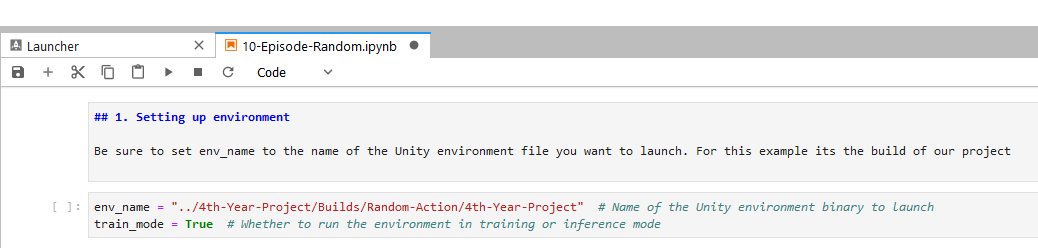
\includegraphics[width=115mm, height=30mm]{img/Notebook1.PNG}
    \caption{Notebook cells before execution}
    \label{fig:sd4}
\end{figure}

\begin{flushleft}
As you can see the first cell block contains the markdown syntax and the second cell containing python syntax before they have been executed.
\end{flushleft}

\begin{figure}[H]
    \centering
    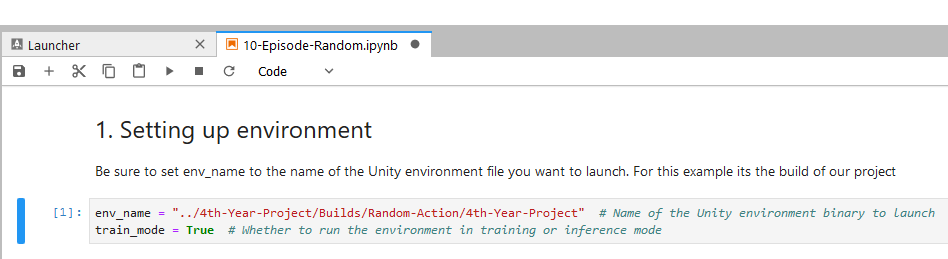
\includegraphics[width=115mm, height=30mm]{img/Notebook2.PNG}
    \caption{Notebook cells after execution}
    \label{fig:sd4}
\end{figure}

\begin{flushleft}
In this image we see both cells after being executed. The number "1" to the left of the cell indicates that this has finished running and its the first python cell that has been executed in the notebook. 
\end{flushleft}

%end

\section{XML}
Here's some nicely formatted XML:
\begin{minted}{xml}
<this>
  <looks lookswhat="good">
    Good
  </looks>
</this>
\end{minted}